\section{Tiền Xử Lý Dữ Liệu}
\subsection{Ghép dữ liệu}
\noindent
Trước hết, nhóm cần cài đặt các thư viện cần được sử dụng trong suốt quá trình làm sạch và xử lý dữ liệu.

\begin{lstlisting}[language=R, caption=Ghép dữ liệu trong R]
required_packages <- c("this.path", "dplyr", "ggplot2", "lubridate", "geosphere", "readr", "corrplot", "faraway", "car", "ggthemes","gt","nortest","knitr","FSA","ggcorrplot","dunn.test")
for (p in required_packages) {
  if (!require(p, character.only = TRUE)) install.packages(p)
  library(p, character.only = TRUE)
}
# Load đường dẫn hiện tại của thư mục data chứa các file CSV mẫu
setwd(this.path::here())
dirty_data <- read_csv("data/dirty_data.csv")
missing_data <- read_csv("data/missing_data.csv")
# Chuyển định dạng tháng ngày năm cột date
dirty_data$date <- parse_date_time(dirty_data$date, orders = c("mdy", "ymd", "dmy"))
missing_data$date <- parse_date_time(missing_data$date, orders = c("mdy", "ymd", "dmy"))
merged_data <- rbind(dirty_data, missing_data)
\end{lstlisting}

\begin{figure}[!ht]
    \centering 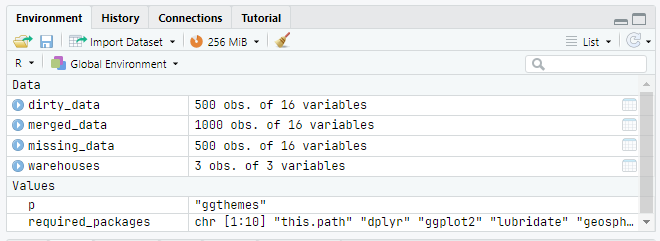
\includegraphics{Images/img/4.0_prepare_data/4.0_after_merge_files.PNG}
    \caption{Sau khi gộp 2 files CSV}
\end{figure}
\begin{boxH}
\textbf{Giải thích:} Thư viện \textbf{this.path} giúp tự động cập nhật đường dẫn thư mục gốc của dự án tại nơi chứa file R. Sau khi tải dữ liệu từ các file CSV mẫu, nhóm gộp hai file này thành một bảng duy nhất để thuận tiện xử lý.    
\end{boxH}
\subsection{Xác định Dữ liệu Khuyết}

Trong quá trình phân tích dữ liệu mẫu, nhóm đã tiến hành kiểm tra sự tồn tại của các giá trị bị khuyết (NA) trong bộ dữ liệu. Kết quả cho thấy một số cột có chứa giá trị khuyết, cụ thể như sau:

\begin{lstlisting}[language=r,caption={Các cột dữ liệu chứa giá trị bị khuyết}]
> na_cout<- colSums(is.na(merged_data ))
> print(na_cout)
                     order_id                   customer_id                          date 
                            0                             0                             0 
            nearest_warehouse                 shopping_cart                   order_price 
                           10                             0                            10 
             delivery_charges                  customer_lat                 customer_long 
                            0                            10                            10 
              coupon_discount                   order_total                        season 
                            0                            10                            10 
        is_expedited_delivery distance_to_nearest_warehouse        latest_customer_review 
                            0                            10                             0 
            is_happy_customer 
                           10 
\end{lstlisting}
\begin{boxH}
    Để phục vụ mục đích làm bài tập lớn và vẽ đồ thị, nhóm đã quyết định bỏ đi ba cột \textbf{distance\textunderscore{to}\textunderscore{nearest}\textunderscore{warehouse}} , \textbf{customer\textunderscore{long}} và \textbf{customer\textunderscore{lat}} và \textbf{nearst\textunderscore{warehouses}}.
\end{boxH}
\subsection{Làm sạch dữ liệu}
\subsubsection{Order\textunderscore{price}, Order\textunderscore{Total}}
Để xử lý các giá trị bị khuyết ở hai cột \textbf{order\_price} và \textbf{order\_total}, nhóm áp dụng công thức:

\begin{equation}
\textbf{order\_total} = \frac{\textbf{order\_price} \times (100 - \textbf{coupon\_discount})}{100} + \textbf{delivery\_charges}
\end{equation}
\noindent
\begin{equation}
\noindent
\textbf{order\_price} = \frac{(\textbf{order\_total} - \textbf{delivery\_charges}) \times 100}{100 - \textbf{coupon\_discount}}
\end{equation}



\begin{lstlisting}[language=R, caption=Xử lý cột \textbf{order\_total} và \textbf{order\_price}]
merged_data <- merged_data %>%
  mutate(
    order_total = ifelse(is.na(order_total), order_price * (100 - coupon_discount) / 100 + delivery_charges, order_total),
    order_price = ifelse(is.na(order_price), (order_total - delivery_charges) * 100 / (100 - coupon_discount), order_price)
  )

\end{lstlisting}
\textbf{Giải thích:} Hàm \textbf{mutate} của thư viện \textbf{dplyr} được sử dụng để thêm hoặc cập nhật cột trong bảng dữ liệu.

\subsubsection{season}

Ở cột \textbf{season}, nhóm nhận thấy một số giá trị không đồng nhất về cách viết hoa hoặc viết thường, dẫn đến dữ liệu thiếu đồng bộ được thể hiện dưới đây:

\begin{lstlisting}[language=R, caption=Giá trị cột \textbf{season} ban đầu]
season_unique_before<-unique(merged_data$season)
print(season_unique_before)

\end{lstlisting}

\begin{lstlisting}[language=R, caption=Xử lý cột \textbf{season}]
merged_data$season <- tolower(merged_data$season) # Đổi tất cả giá trị mùa dạng viết thường
month_value <- month(merged_data$date) # lấy tháng trong cột $date
merged_data <- merged_data %>%
  # Toán tử %>% : Truyền kết quả của phép toán hoặc hàm vào hàm tiếp theo .
  # mutate: Tạo ra cột mới hoặc thay đổi giá trị các cột trong data frame
  mutate(season = case_when(
    !is.na(season) ~ season,
    month_value %in% c(12, 1, 2) ~ "winter",
    month_value %in% c(3, 4, 5) ~ "spring",
    month_value %in% c(6, 7, 8) ~ "summer",
    TRUE ~ "autumn"
  ))

\end{lstlisting}
\begin{boxH}
\textbf{Giải thích:} Nhóm đã lấy giá trị \textbf{tháng} trong cột \textbf{date} của dữ liệu mẫu và sử dụng hàm \textbf{case\textunderscore{when}} xuất ra mùa và thế vào các giá trị bị khuyết. 
\end{boxH}
\begin{lstlisting}[language=R, caption=Dữ liệu cột \textbf{season} sau khi xử lý]
> season_unique_after<-unique(merged_data$season)
> print(season_unique_after)
[1] "winter" "summer" "autumn" "spring"
\end{lstlisting}

\subsubsection{is\textunderscore{happy}\textunderscore{customer}}
\begin{lstlisting}[language=R, caption=Làm tròn trung vị]
median_happy_customer <- round(median(merged_data$is_happy_customer, na.rm = TRUE), digits = 0)
merged_data$is_happy_customer[is.na(merged_data$is_happy_customer)] <- median_happy_customer
\end{lstlisting}
\begin{boxH} 
\textbf{Giải thích:}
    Lí do nhóm sử dụng giá trị trung vị cho cột 
is\textunderscore{happy}\textunderscore{customer} để \textbf{phản ánh độ hài lòng của khách hàng}, chúng chỉ có rơi vào một trong hai trường hợp là 0 và 1 (Hài lòng hoặc không hài lòng) và không ảnh hưởng bởi các giá trị ngoại lai .
\end{boxH}
\subsubsection{Kiểm tra dữ liệu sau khi làm sạch}
Sau khi dữ liệu được làm sạch, kiểm tra có cột nào còn dính giá trị bị khuyết nữa không.

\begin{lstlisting}[language=R, caption=Kiểm tra dữ liệu bị khuyết sau khi làm sạch]
> na_cout<- colSums(is.na(merged_data ))
> print(na_cout)
                     order_id                   customer_id                          date 
                            0                             0                             0 
            nearest_warehouse                 shopping_cart                   order_price 
                           10                             0                             0 
             delivery_charges                  customer_lat                 customer_long 
                            0                            10                            10 
              coupon_discount                   order_total                        season 
                            0                             0                             0 
        is_expedited_delivery distance_to_nearest_warehouse        latest_customer_review 
                            0                            10                             0 
            is_happy_customer 
                            0 
> 
\end{lstlisting}

% Xong phần làm sạch dữ liệu